\documentclass[a4paper,12pt]{article}
%%%%%%%%%%%%%%%%%%%%%%%%%%%%%%%%%%%%%%%%%%%%%%%%%%%%%%%%%%%%%%%%%%%%%%%%%%%%%%%%%%%%%%%%%%%%%%%%%%%%%%%%%%%%%%%%%%%%%%%%%%%%%%%%%%%%%%%%%%%%%%%%%%%%%%%%%%%%%%%%%%%%%%%%%%%%%%%%%%%%%%%%%%%%%%%%%%%%%%%%%%%%%%%%%%%%%%%%%%%%%%%%%%%%%%%%%%%%%%%%%%%%%%%%%%%%
\usepackage{eurosym}
\usepackage{vmargin}
\usepackage{amsmath}
\usepackage{graphics}
\usepackage{epsfig}
\usepackage{enumerate}
\usepackage{multicol}
\usepackage{subfigure}
\usepackage{fancyhdr}
\usepackage{listings}
\usepackage{framed}
\usepackage{graphicx}
\usepackage{amsmath}
\usepackage{chngpage}
%\usepackage{bigints}

\usepackage{vmargin}
% left top textwidth textheight headheight
% headsep footheight footskip
\setmargins{2.0cm}{2.5cm}{16 cm}{22cm}{0.5cm}{0cm}{1cm}{1cm}
\renewcommand{\baselinestretch}{1.3}

\setcounter{MaxMatrixCols}{10}

\begin{document}
\large

\subsection*{Exercise 1}
\noindent The following data represent the average total number of marks obtained for a
particular exam, observed over seven exam sessions that had been administered by a
professional examination body:


\[87, 53, 72, 90, 78, 85, 83 \]

\noindent Enter these data into R and compute their sample mean and variance.




\begin{framed}\begin{verbatim}
y <- c(87, 53, 72, 90, 78, 85, 83)

mean(y)

c(mean=mean(y), variance=var(y)) 
\end{verbatim}\end{framed}


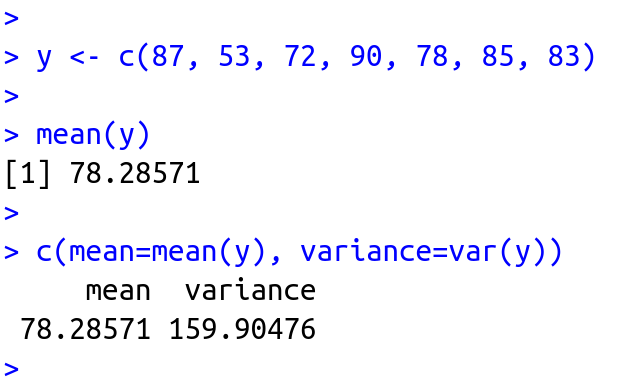
\includegraphics[scale=0.45]{00-A1/images/A1-Q1.png}


%%%%%%%%%%%%%%%%%%%%%%%%%%%%%%%%%%%%%%%%%%%%%%
\newpage 
\subsection*{Exercise 2}

\noindent Investigate whether the Poisson model is appropriate for these data, by calculating the sample mean and sample variance of 10 Poisson samples
having the same size and mean as the sample given above.\\
\medskip

\noindent \textbf{Recall:}\\

\noindent For the Poisson distribution $$ E(X)  = Var(X)$$



\begin{framed}\begin{verbatim}
xbar = s2 = numeric(10)

xbar
s2
\end{verbatim}\end{framed}


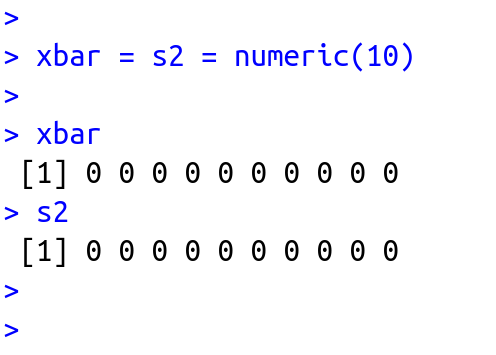
\includegraphics[scale=0.45]{00-A1/images/A1-Q1-ForLoop-1.png}

%%%%%%%%%%%%%%%%%%%%%%%%%%%%%%%%%%%%%%%%%%%%%%%%%%%%
\newpage 
\noindent use \texttt{rpois()} to generate 7 random numbers.


\begin{framed}\begin{verbatim}
x <- rpois(7, lambda= 78.29)
x
\end{verbatim}\end{framed}


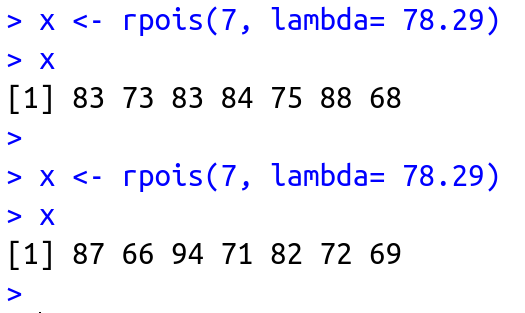
\includegraphics[scale=0.45]{00-A1/images/A1-Q1-rpois.png}

\newpage 


\begin{framed}\begin{verbatim}

set.seed(1234)

for (j in 1:10){

    x <- rpois(7, 78.29)
 
    xbar[j] <- mean(x)
 
    s2[j] <- var(x)

}

\end{verbatim}\end{framed}

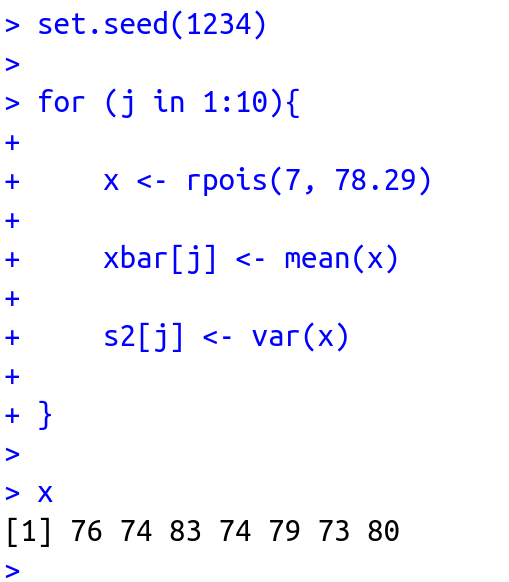
\includegraphics[scale=0.45]{00-A1/images/A1-Q1-ForLoop.png}

\newpage 


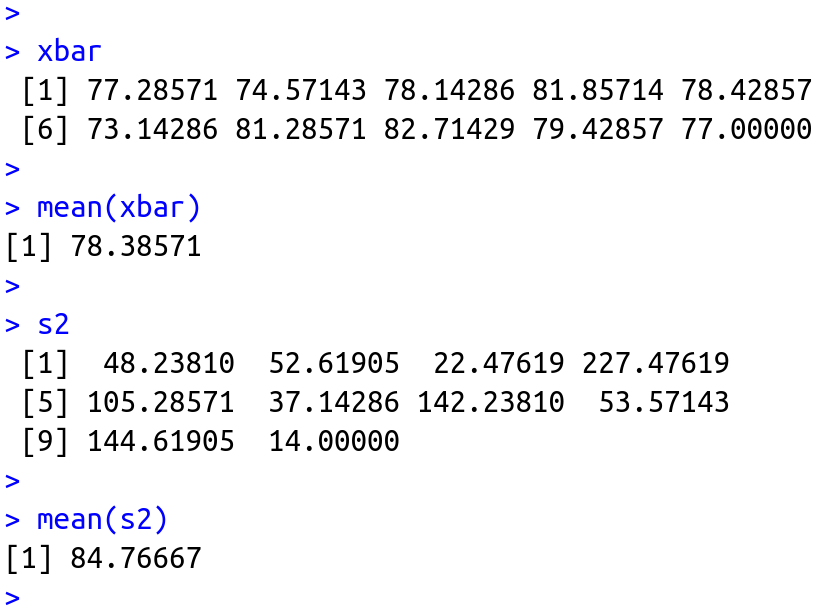
\includegraphics[scale=0.45]{00-A1/images/A1-Q1-Estimates.png}



\noindent It is unusual to get as large a difference between the mean and the variance as that observed for these data, 
making it doubtful that these data are from a Poisson distribution. 
%%%%%%%%%%%%%%%%%%%%%%%%%%%%%%%%%%%%%%%
\newpage 
\subsection*{Exercise 3}

\noindent Investigate whether the Poisson model is appropriate for these data, by calculating the sample mean and sample variance of 10,000 Poisson samples
having the same size and mean as the sample given above.


\newpage 

\begin{framed}
\begin{verbatim}
set.seed(1234)

for (j in 1:10000){

    x <- rpois(7, 78.29)
 
    xbar[j] <- mean(x)
 
    s2[j] <- var(x)

}


hist(xbar, breaks = 200,col="lightblue" )
 
hist(s2, breaks = 200,col="pink" )

\end{verbatim}
\end{framed}

\newpage 


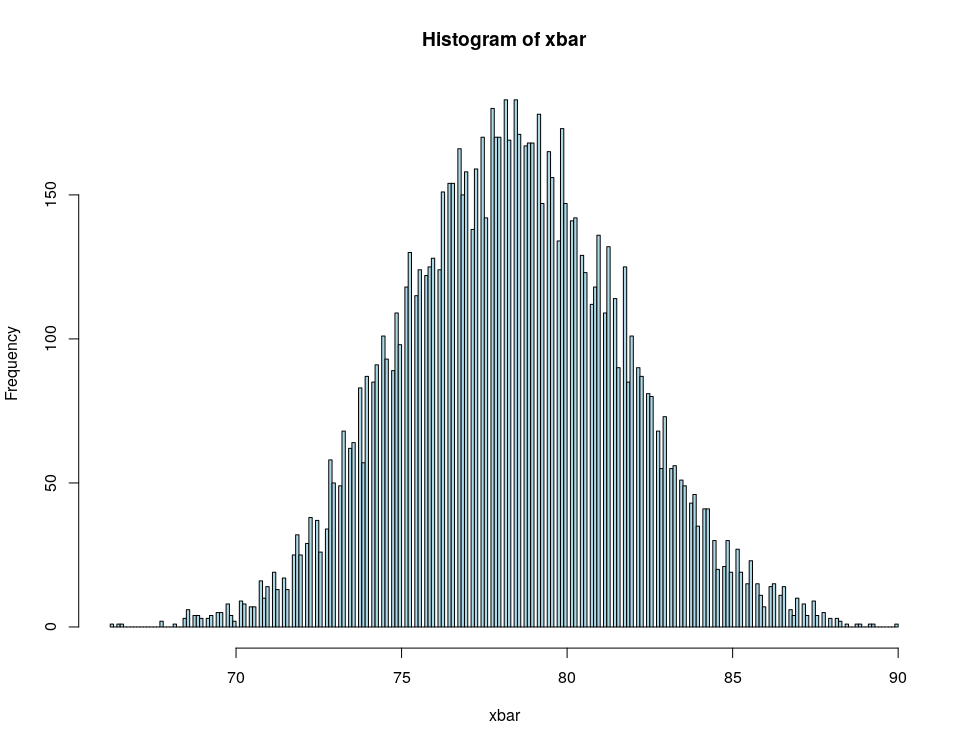
\includegraphics[scale=0.48]{00-A1/images/AA-Q1-Hist-Xbar.png}

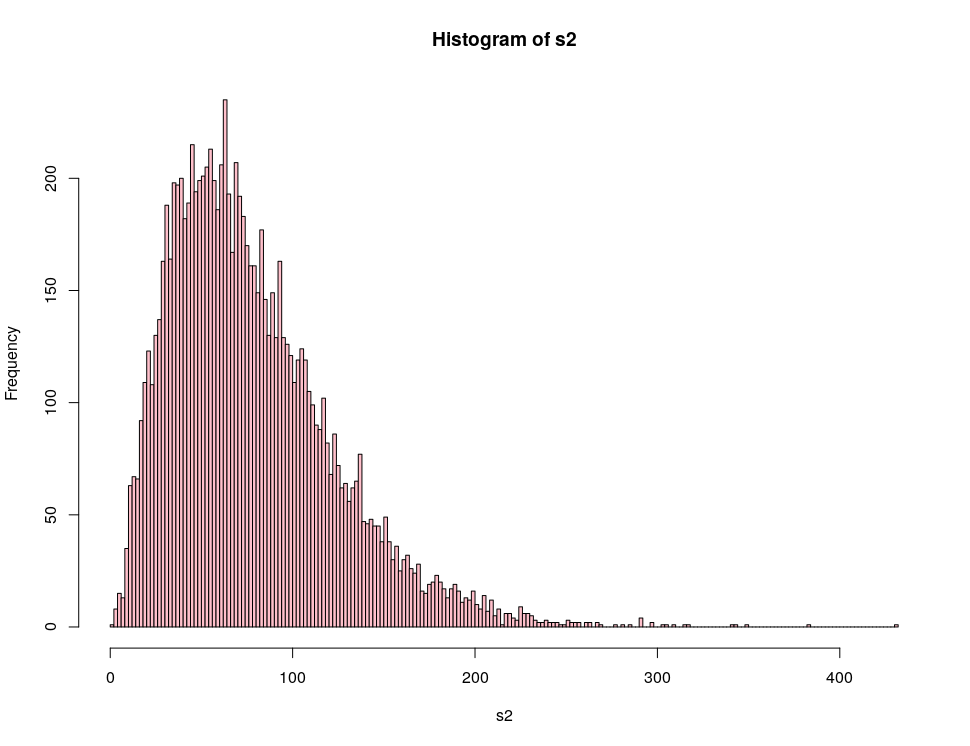
\includegraphics[scale=0.48]{00-A1/images/A1-Q1-Hist-S2.png}




%%%%%%%%%%%%%%%%%%%%%%%%%
\newpage 




\begin{framed}\begin{verbatim}
mean(s2>159)
\end{verbatim}\end{framed}




\end{document}
